\documentclass[class=article,border=5pt,tikz]{standalone}
\usepackage{fontawesome}% \faScissors

\begin{document}
  \begin{tikzpicture}[thick,scale=2.5,font=\large]
  \begin{scope}
    \draw[ultra thick] (0,0)--++(1,0)--++(0,1)--++(-1,0) node[midway,above] {Figure A} --cycle;
    \draw[dotted,gray](0,0.5)--++(1,0);
    \draw[dotted,gray](0.5,0)--++(0,1);
  \end{scope}
  \begin{scope}[shift={(2cm,0)},scale=0.5]
    \draw[ultra thick] (0,0)--++(1,0)--++(0,1);
    \draw[dashed,gray] (1,1)--++(-1,0) node[black,midway,above,yshift=1.27cm] {Figure B} --++(0,-1);
  \end{scope}
  \begin{scope}[shift={(4cm,0)},scale=0.5]
    \draw[ultra thick] (0,0)--++(1,0)--++(0,1);
    \draw[dashed,gray] (1,1)--++(-1,0) node[black,midway,above,yshift=1.27cm] {Figure C} --++(0,-1);
    \draw[dashed,fill=gray] (0,0)--++(0.5,0.5)--++(0.5,-0.5);
    \node at (-3pt,0) {\huge\faScissors};
  \end{scope}
  \end{tikzpicture}
\end{document}

